% energyL22.tex
% $Author$ $Date$

% \subsection{Symmetry invariant moments for $L=22$} % of the \KSe}
% \label{sec:energyL22}
% Predrag                   May 1 2007

%%%%%%%%%%%%%%%%%%%%%%%%%%%%%%%%%%%%%%%%%%%%%%%%%%%%%%%%%%%%%%%%
\begin{figure}[t]
\begin{center}
(a)\!\!\!\!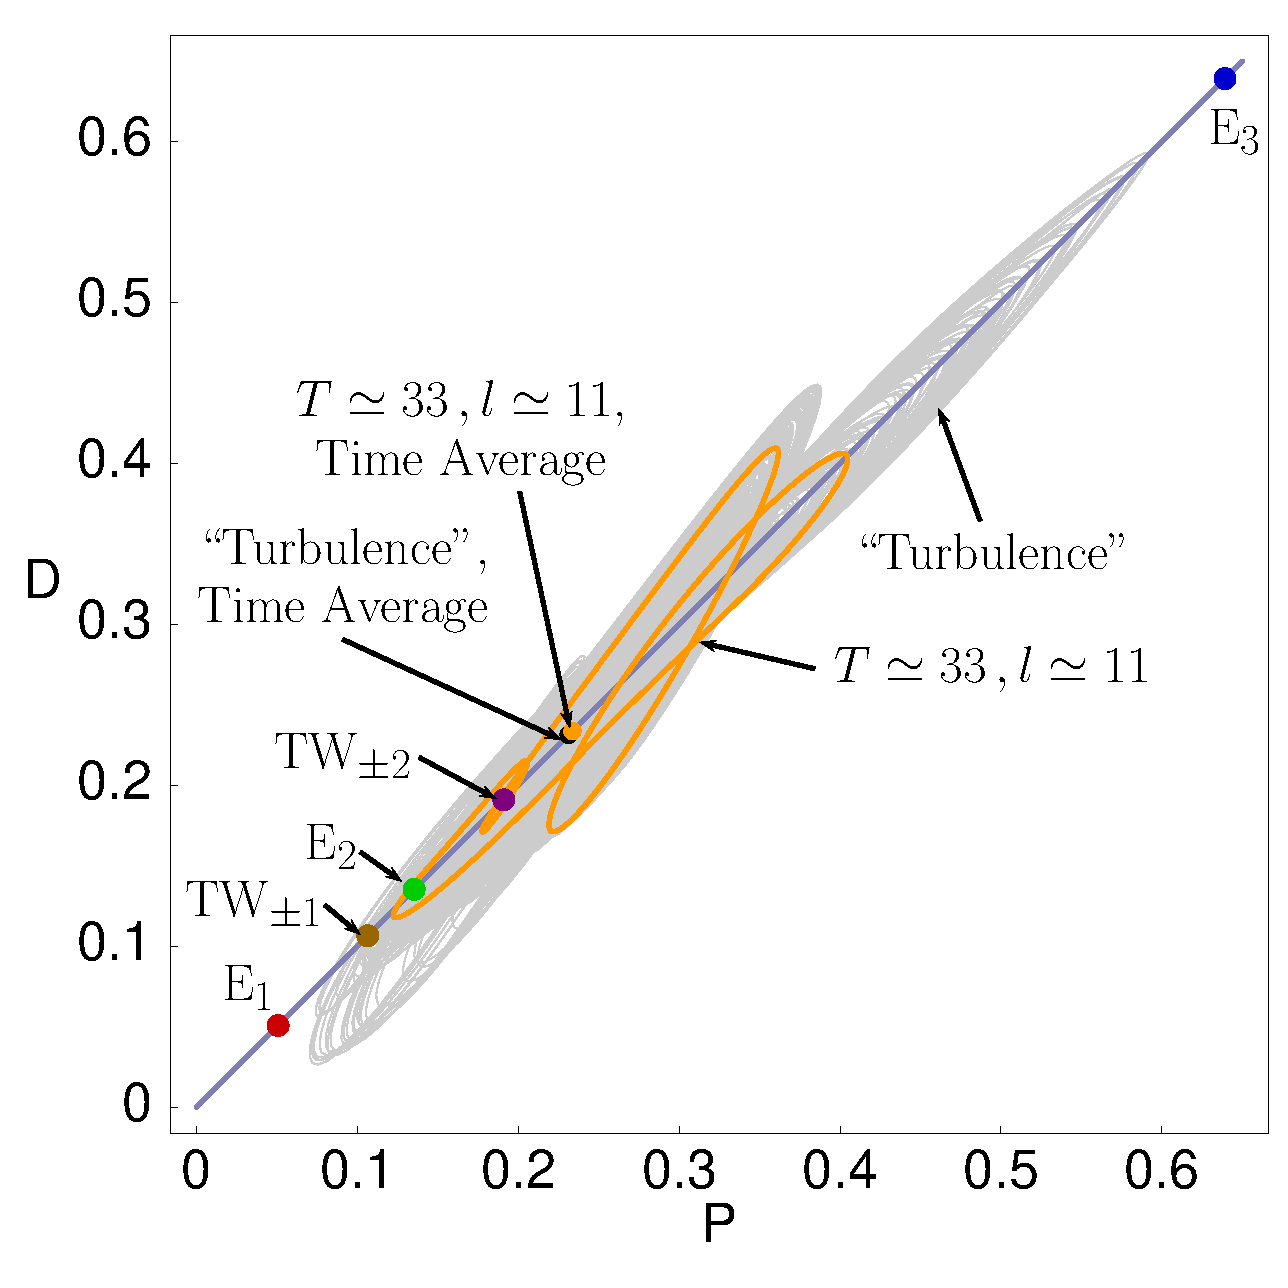
\includegraphics[width=0.48\textwidth]{figs/energyBalance_pst.eps}%
~(b)\!\!\!\!\includegraphics[width=0.48\textwidth]{figs/EDequiva_pst.eps}
\end{center}
\caption{
(a) Power input $P$ {\em vs.}
dissipation rate $D$
(b) energy $E$  {\em vs.}
dissipation rate $D$,   for several  \eqva\ and \reqva,
a \rpo , and a typical `turbulent' long-time trajectory.
System size $L=22$.
        }
\label{f:drivedrag}
\end{figure}
%%%%%%%%%%%%%%%%%%%%%%%%%%%%%%%%%%%%%%%%%%%%%%%%%%%%%%%%%%%%%%%%%%

%%%%%%%%%%%%%%%%%%%%%%%%%%%%%%%%%%%%%%%%%%%%%%%%%%%%%%%%%%%%%%%%
\begin{figure}[t]
\begin{center}
(a)\!\!\!\!\includegraphics[width=0.48\textwidth]{figs/ks22TurbConn_xfig.eps}%
~~(b)\!\!\!\!\includegraphics[width=0.48\textwidth]{figs/ks22TurbConn_xfig.eps}
\end{center}
\caption{
Two projections of the $(E,P,\dot{E})$ representation of the flow.
\EQV{1} (red), \EQV{2} (green), \EQV{3} (blue),
connections from \EQV{1} to $A(L/4)\EQV{1}$ (green),
from $A(L/4)\EQV{1}$ to \EQV{1} (yellow-green)
and from \EQV{3} to $A(L/4)\EQV{1}$ (blue), superimposed over
a generic long-time `turbulent' trajectory (grey).
System size $L=22$.
        }
\label{f:drivedragConn}
\end{figure}
%%%%%%%%%%%%%%%%%%%%%%%%%%%%%%%%%%%%%%%%%%%%%%%%%%%%%%%%%%%%%%%%%%

\PC{
 Implementing Ruslan: all axes in \reffig{f:drivedragConn} changed by a factor
of 2?
        \\
Implementing Predrag:
label axes in \reffig{f:drivedrag}, \reffig{f:drivedragConn}
by $(E,P,D,\dot{E})$
    }
\PC{ks22TurbConn2\_xfig.eps for \reffig{f:drivedragConn}
    not checked in?
   }
\PC{\refFig{f:drivedragConn}: split into three figures, \\
    (a) label axes $(E,P)$, move to \reffig{f:drivedrag}\,(\textit{b})\\
    (b) flip $y$ axis as $\dot{E}=P-D$; label axes $(P,\dot{E})$ \\
    (c) flip $y$ axis; label axes $(E,\dot{E})$ \\
   }
In \reffig{f:drivedrag}
we plot \refeq{EnRate}, the time-dependent $\dot{\expctE}$
in the
power input $P$ {\em vs.} %$\expct{u_{x}{}^2}$ vs.
dissipation rate $D$ %$\expct{u_{xx}{}^2}$
plane, for all $L=22$ \eqva\ and
\reqva\ \PCedit{determined so far},
several \po s and \rpo s, and for a typical `turbulent'
long-time trajectory.
\PC{\reffig{f:drivedrag}:
%    (0) replace $y$-axis by
%    $\expct{(u_{xx})^2}-\expct{(u_{x})^2}$, so all \po s lie
%    on the $x$-axis and on can see more clearly the turbulent and
%    periodic trajectory, instead having them scrunched into the
%    diagonal. (a) Replace by side views of
%    3-$d$ $(\expct{u^2},\expct{(u_{x})^2},\expct{(u_{xx})^2}
%       -\expct{(u_{x})^2})$,
%    two figures;
    (b) current type figure, with chaotic trajectory,
    all \eqva, $(32.\cdots,11)$ as example of well embedded, and
    a typical \po\ {\em not} embedded into the `turbulent' attractor.
    (c) a separate figure with more \po s, no `turbulent' attractor.
%    (d) prepare a mathematica macro that automatically uses
%    fonts at least twice the size you use currently.
    (e) replace
    gray window with a white background, black font. (f) in the
    publication version replace colored dots with symbols of varying
    shapes, fine black border, can be filled in with colors.
    }

Projections
from the $\infty$-dimensional \statesp\ onto
the 3-dimensional
$(E,P,D)$ representation of the flow, such as
\reffigs{f:drivedrag}{f:drivedragConn},
can be misleading.
Another example is the \rpo\ $(\period{p},\shift_p) =(32.8,10.96)$
which appears well embedded within the turbulent flow.
The mean value of $\timeAver{P_p}$
evaluated on it,
\reffig{f:ks22rposShort}\,(\textit{c}),
is quite close to the long-time turbulent
time average $\timeAver{P}$.
Similarly close prediction of mean dissipation rate in the
\pCf\ from a single-period \po\ computed by
Kawahara and Kida\rf{KawKida01} has lead to
optimistic hopes that `turbulence' is different from
low-dimensional chaos, insofar that the determination of one
magic \po\ could yield all long-time predications.
Regrettably, not true - as always, here too one needs a hierarchy
of \po s of increasing length to obtain accurate
predictions\rf{DasBuch}.
% \PC{\PCedit{ the Japanese heresy disposed off}}

The most one can say is that if points are clearly separated in an
$(E,P,D)$ plot (for example, in \reffig{f:ks22rposShort}
$\EQV{1}$ \eqv\ is not part of the recurrent set), they are also separated
in the full \statesp. Converse is not true - states of
very different topology can have similar energies.
